%% Languages: norsk				
%%						english			
%% Styles:		twoside, 		The margins will differ dependent on right/left pages
%%						openright		The first page is a "right" page
%% indexes:		listings		Show figure list, table list
%%						glossary		Show glossary and abbreviation list
%%						todo				Show list of todo-notes in documents
%%						%
\documentclass[english]{gucreport}
\input{gucreport}

\begin{document}
	%\input{glossary}
	\makefrontpages
	\tableofcontents
	\showindex		%%lists of figures, codes, tables, glossary, etc
	
	%% Chapters for the text
	
\chapter{Task A}
\section{Environment description}
The environment is implemented as a weighted, un-directed graph, figure
\ref{fig:graph}.  The graph consist of Vertices(figure \ref{fig:vert}) and
Edges(figure \ref{fig:edge}) that is connected to each other.  By doing this we
can let the agent traverse the graph by itself using an implementation of the
shortest path algorithm as the heuristic for the A* algorithm to select the next
move to make. 

The environment also contains the possibility for marking edges as broken,
vertices as visited, and creating edges between Vertices.

\begin{figure}[h]\centering
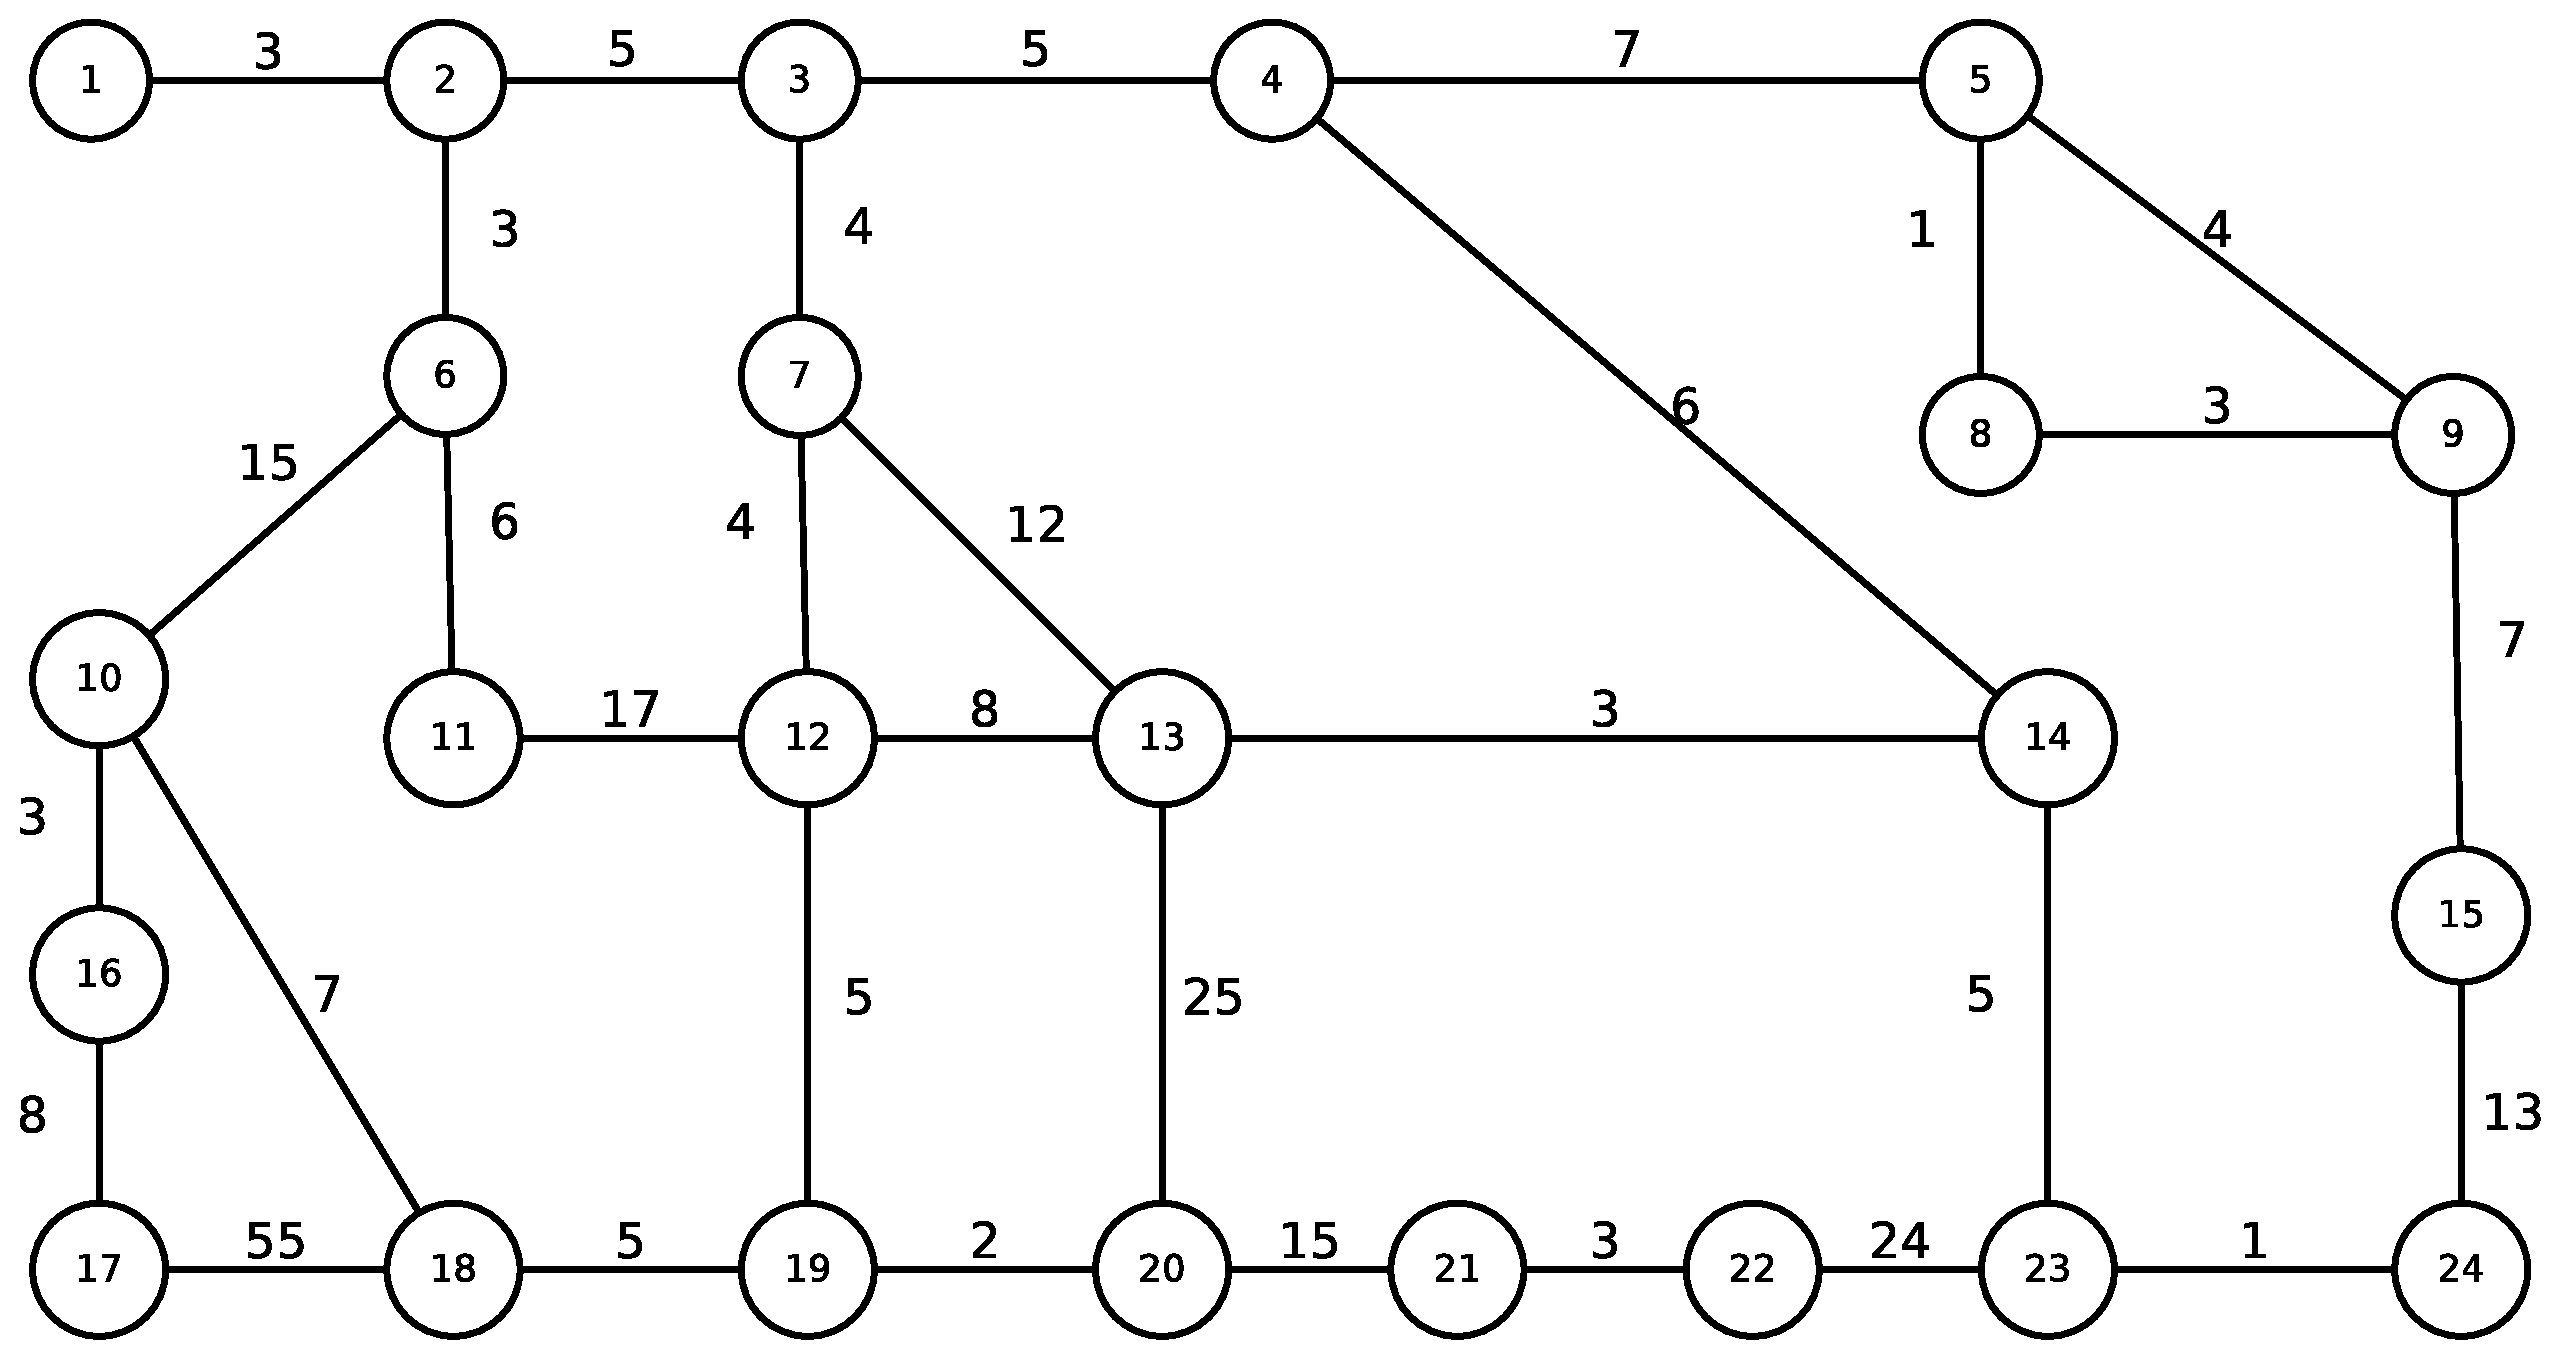
\includegraphics[ width={0.7\textwidth} ]{pictures/graph}
\caption{The environment - A non-directed graph with weighted edges.}
\label{fig:graph}
\end{figure}


\subsection{Creationism}
As the program starts up we read the file "vertice.lst" which contains a number
stating how many vertices are going to be in the graph. After reading this
integer we continue by creating the vertices and adding them to our Vertice
list.

The vertice list is built up using two elements to depict the start and end of
the list. The Vertice object, "vStart", is a dummy-element at the start of the
list. After this element all "real" elements follows.  Finally the last "real"
element is linked to the Vertice object "vTail", which represent the end of the
list.

The vertice list is represented in figure \ref{fig:vertlst}. The vStart object
is the start of the list, but holds no value other than a link to the first real
Vertice object. The "real" Vertices will hold different values describing its
state and information.

\begin{figure}[h]\centering
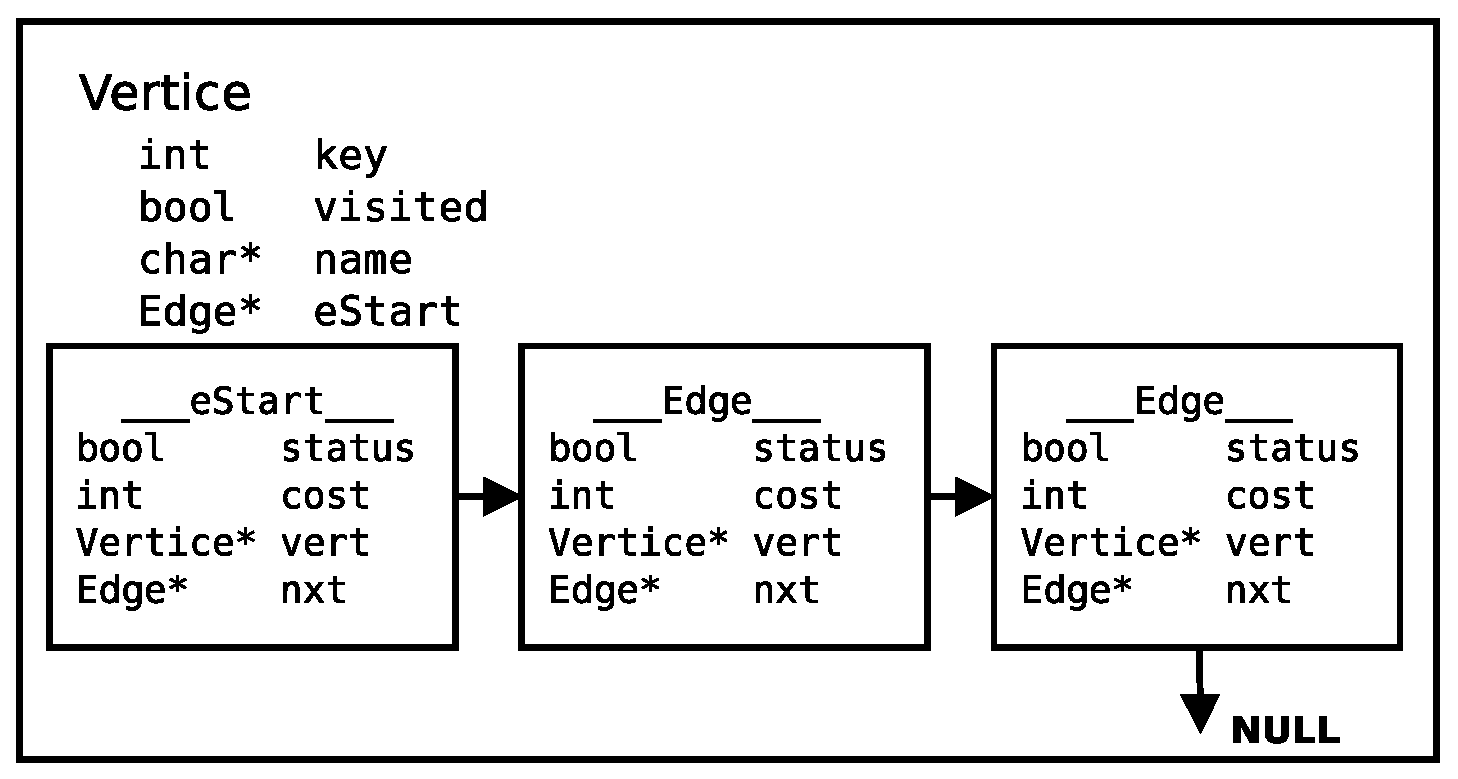
\includegraphics[ width={0.6\textwidth} ]{pictures/data_structure}
\caption{Illustration of the structure of a Vertice object}
\label{fig:vertlst}
\end{figure}

\subsection{Vertice}
\begin{description}
\item [key:]			This is an integer value holding the reference key to the
	Vertice. It is assigned automatically during creation of the vertice using an
	auto incremented counter starting at 1.  This is used to identify a specific
	Vertice in the graph and the vertice list.
\item [name:]			This is an unused variable and is assigned to NULL during
	creation. It is meant to hold a small text describing the name of the Vertice,
	and is usefull if it the graph represents a map or other things that could be
	assigned a description using a name tag.
\item [visited:]	This is a boolean describing wether or not the Vertice has
	been visited. It is not currently used, but could be used to mark a cell as
	visited during traversal.
\item [nxtVert:]	This is a pointer to a Vertice object. This will point to
	either the next Vertice in the list or to the vTail object which represents
	the end of the vertice list.  For vTail this link will link back to itsself.
\item [eStart:]		This is an Edge pointer which is on construction initialized
	to an Edge object that points to NULL.  This edge is the starting element for
	the list of Edges stemming from the current Vertice to adjacent vertices.
	eStart is however a dummy-element that points to the first actual edge in the
	list.
\end{description}
\begin{figure}\centering
	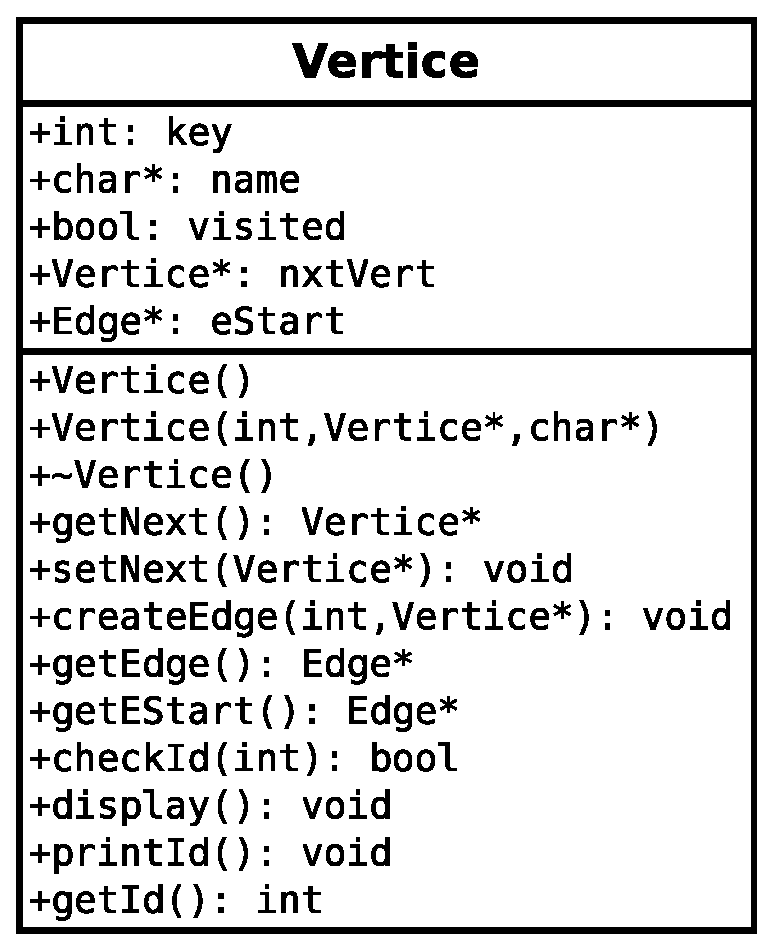
\includegraphics[ width={0.35\textwidth} ]{pictures/uml_vertice}
	\caption{UML description of a Vertice's variables and implemented functions}
	\label{fig:vert}
\end{figure}

\subsection{Edge}

\begin{description}
\item[status:]	This boolean value holds the status of the edge, which means 
	whether or not it	is traversable.  This could be used to update the 
	environment dynamically runtime.
\item[cost:]		This is the integer value representing the cost of traveling the
	edge from current vertice to the linked vertice.
\item[nxt:]			This is the a pointer to the next Edge in the edge list. The
	first edge in the list will be the dummy edge and the last element will point
	to NULL, which will result in a segfault if not handled properly.
\item[vert:]		This is a pointer to the linked Vertice in which the edge links
	to.
\end{description}

\begin{figure}[h]\centering
	\includegraphics[ width={0.35\textwidth} ]{pictures/uml_edge}
	\caption{UML description of an Edge's variables and implemented functions}
	\label{fig:edge}
\end{figure}

\subsection{Vertice List}

\begin{figure}\centering
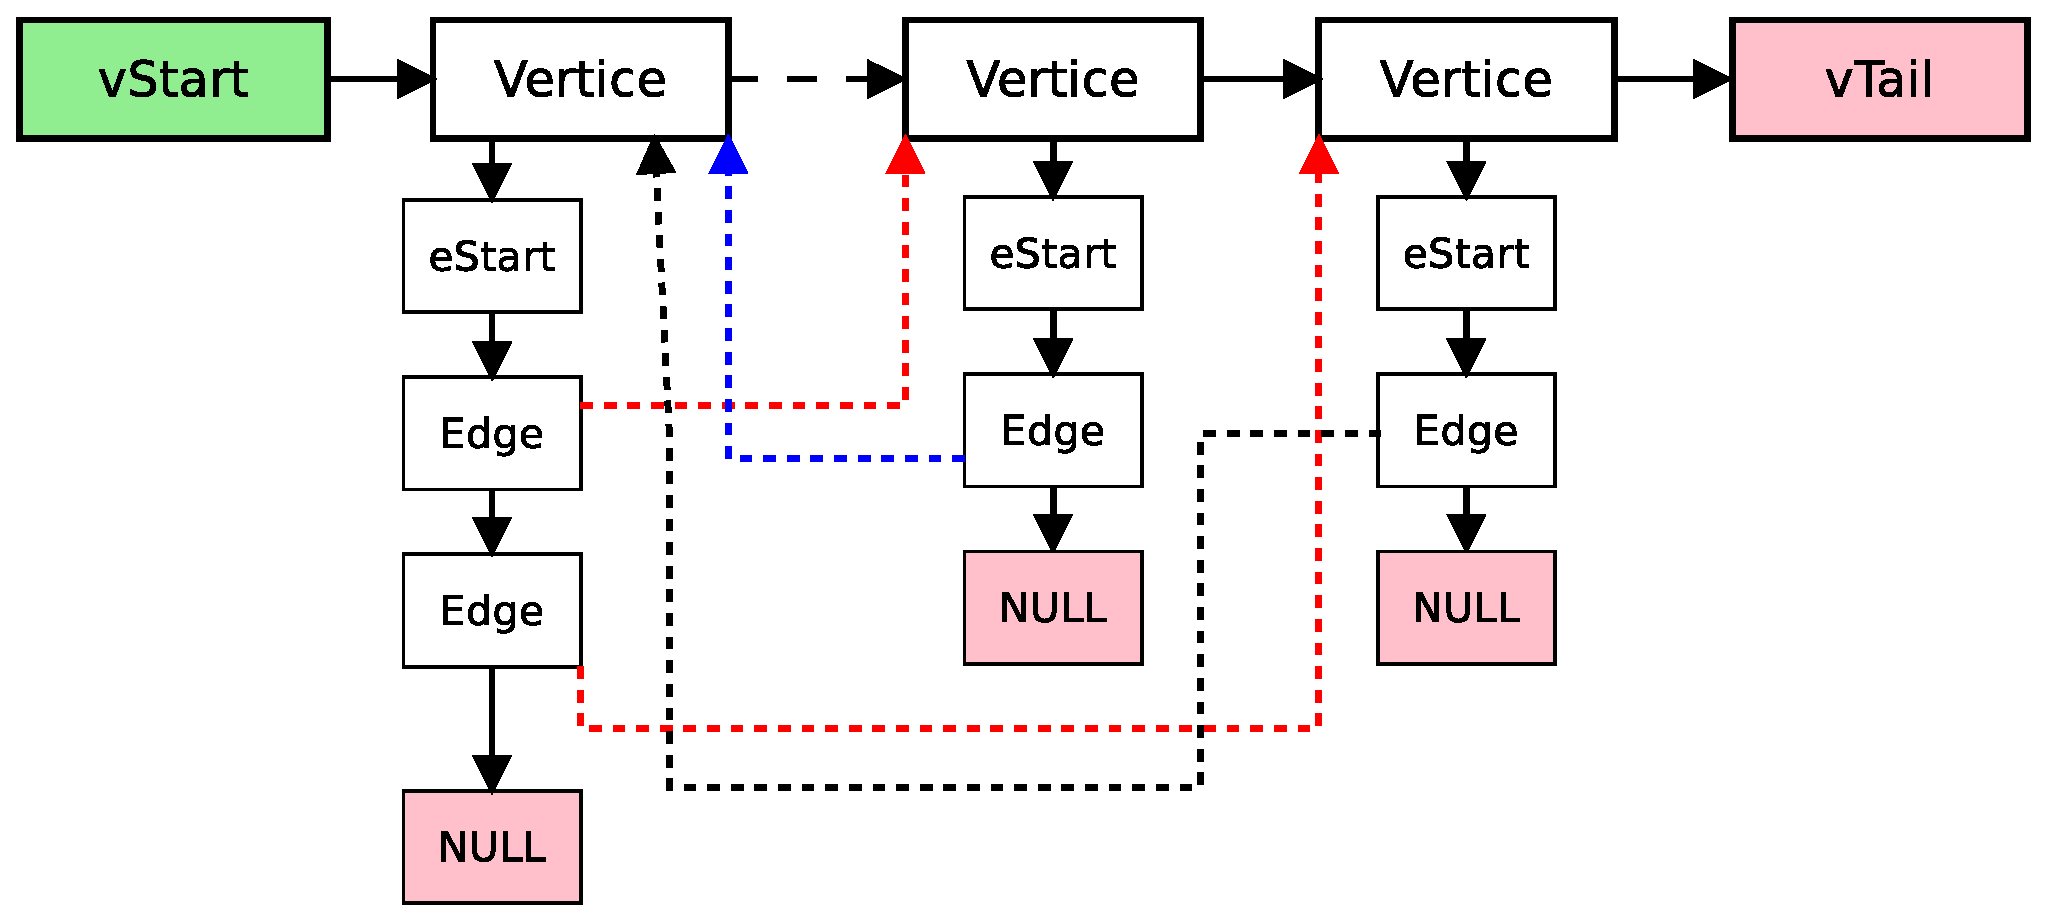
\includegraphics[ width={0.9\textwidth} ]{pictures/vertice_list}
\caption{Illustration of the list holding all the Vertices in the graph
environment}
\end{figure}


\subsection{Fringe List}


\begin{figure}\centering
\includegraphics[ width={0.4\textwidth} ]{pictures/uml_fringe}
\caption{UML description of the Fringe object}
\end{figure}




\section{Agent - A* Tree Search}


\begin{figure}\centering
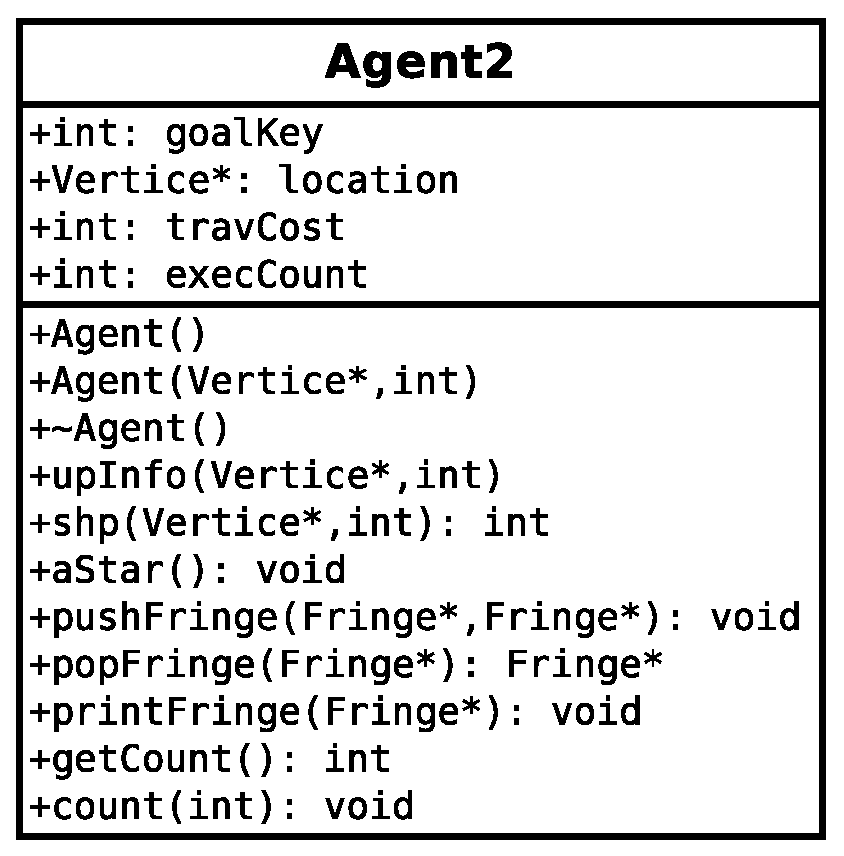
\includegraphics[ width={0.4\textwidth} ]{pictures/uml_agent2}
\caption{UML description of the Agent used for A* tree search}
\end{figure}


\section{A* Star Tree Search algorithm}

\begin{description}
\item[]
\end{description}

\begin{figure}
\centering
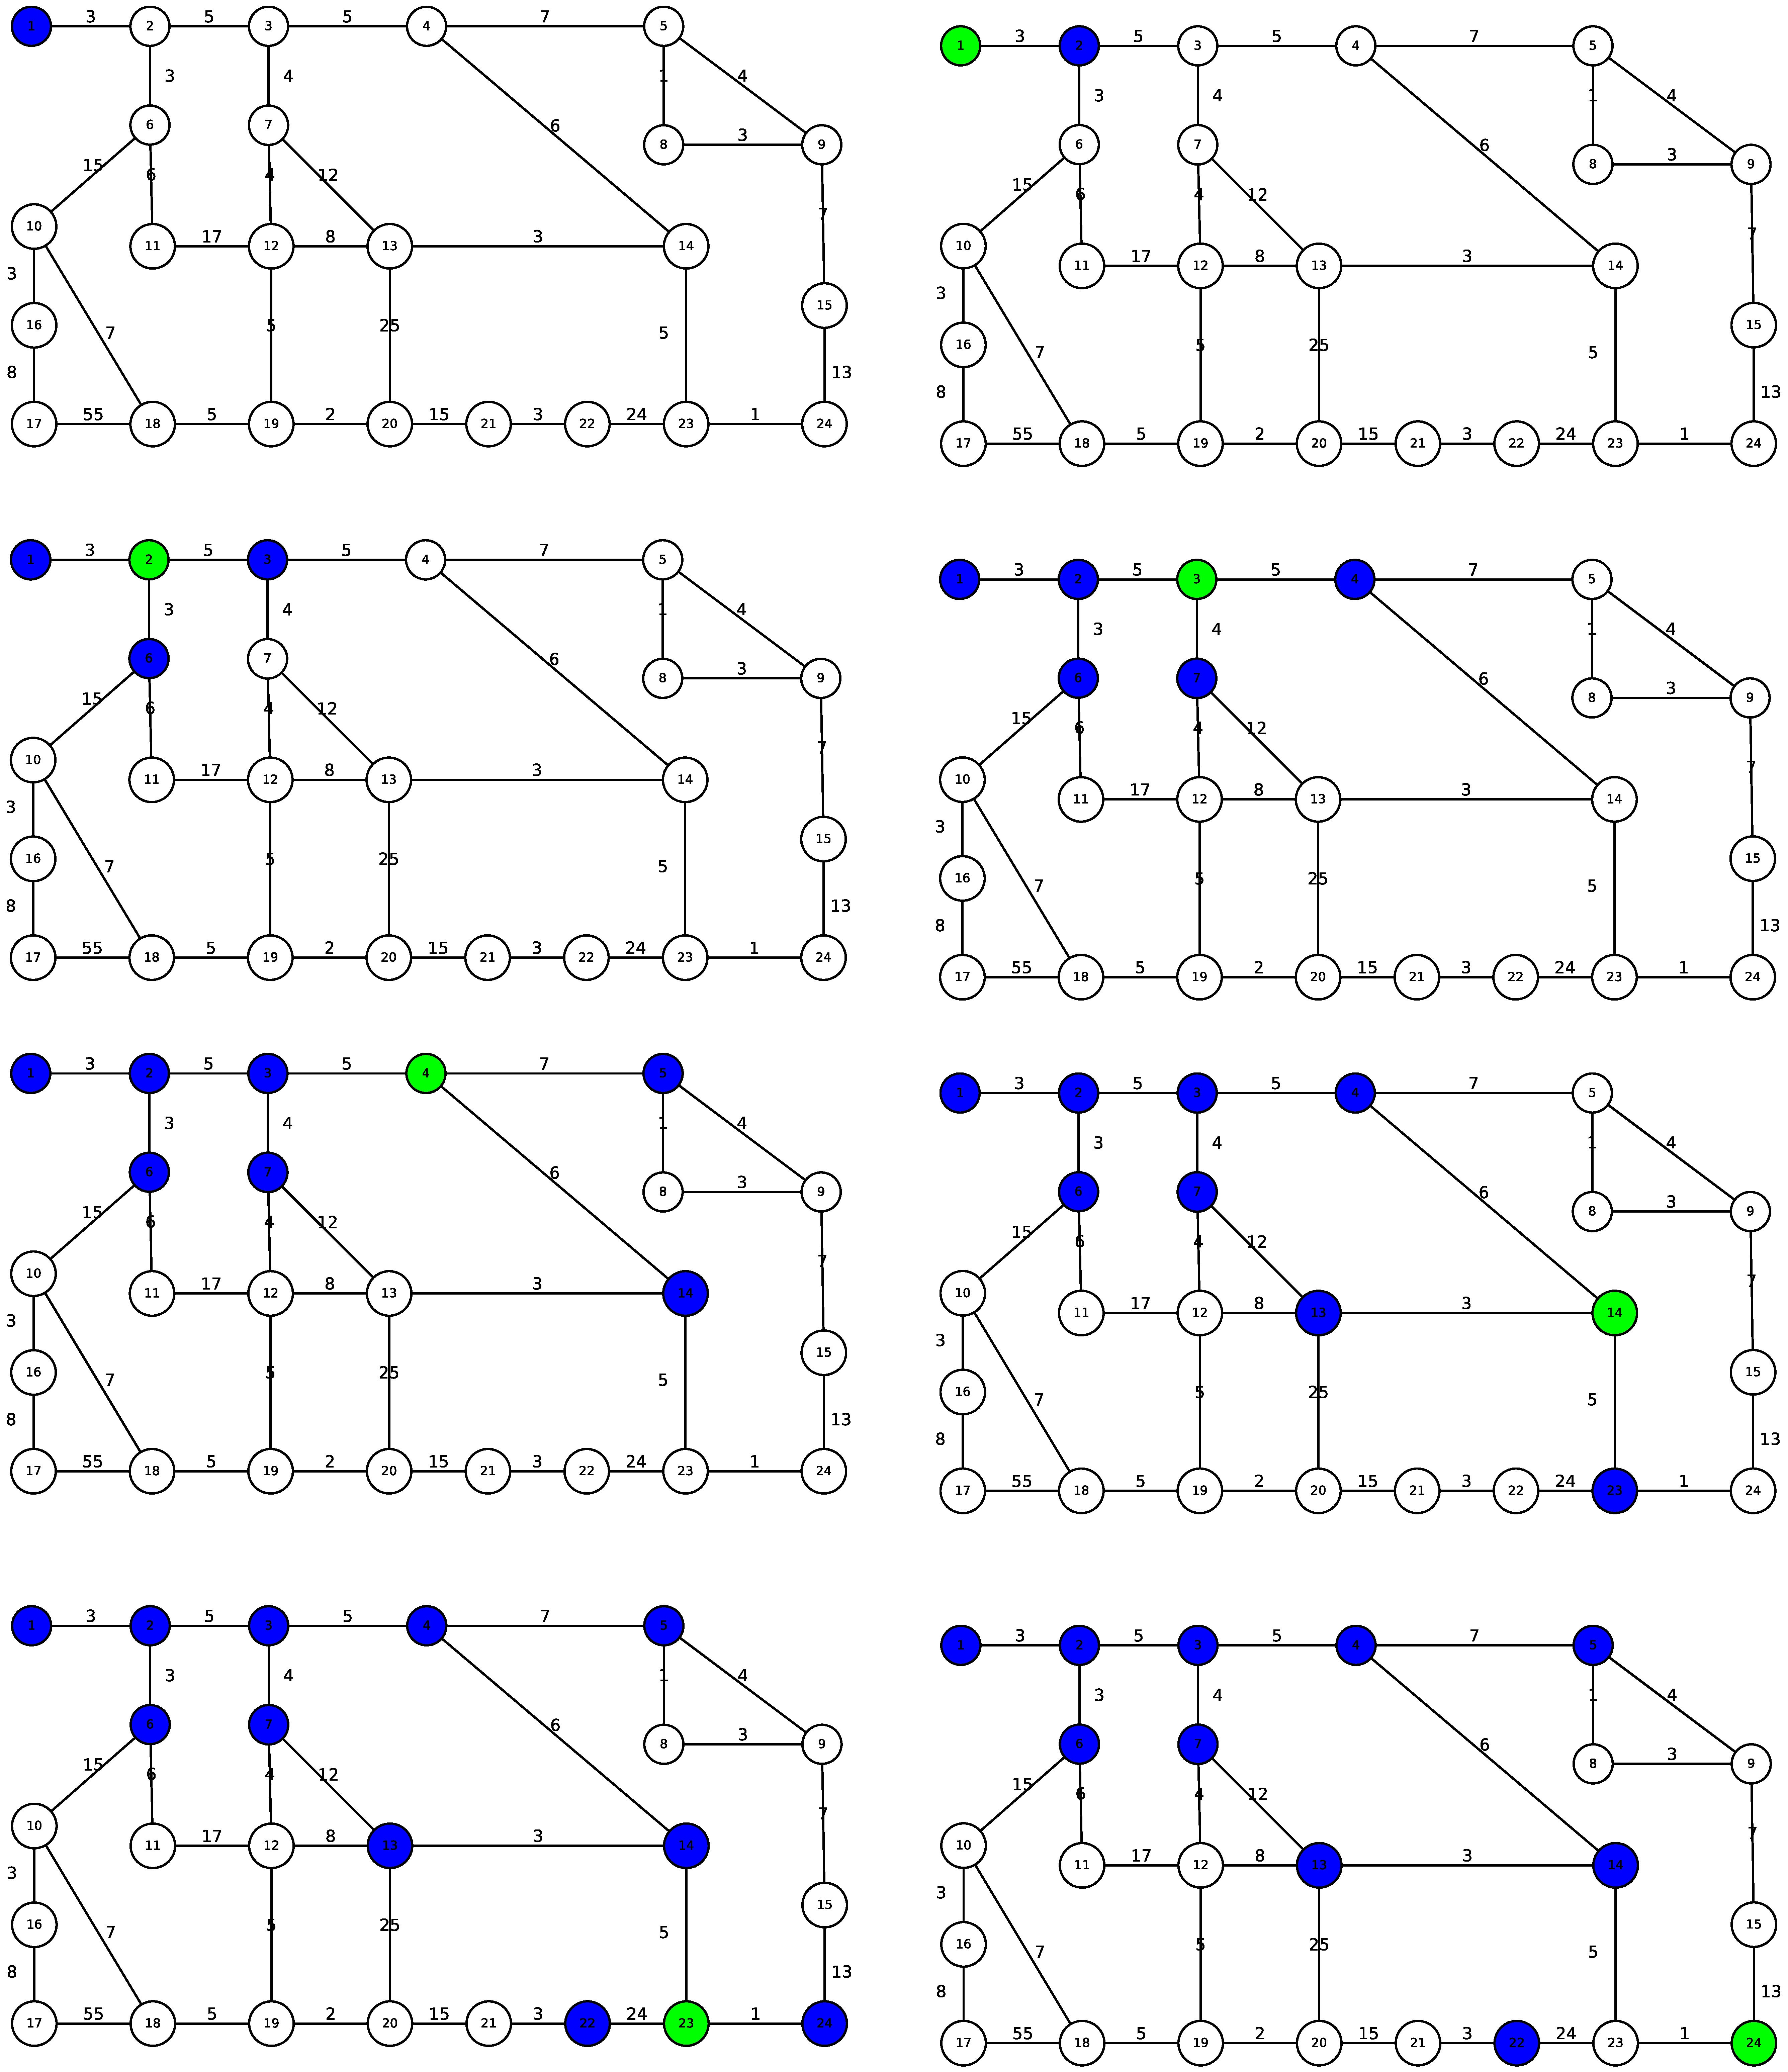
\includegraphics[ width={\textwidth} ]{pictures/tree_search}
\caption{A* star tree search algorithm}
\end{figure}



	
\chapter{Task B}
A* graph search has being implemented on a recursive manner. 
\section{Environment changes}
The main environment will not change from task A. This agent still works on Vertices and Edges. The difference is the way of storing the path. 
The agent in task A stores it in an open list, in the other hand the agent in this case stores the final path in a closed list. The lists 
implemented in this case are bidirectional so the traversal can be done both ways.

\section{Agent description}

The agent contains, as shown on the picture, the following fields:\\
\begin{description}
\item[Fringe:]Open list used in the heuristic, for which we use the shortest path algorithm. The fringe is a pointer to a list of Node, 
a struct described in agent.h and on the picture.
\item[Open:]Open list used in the A* algorithm. It's also a list of Nodes like the fringe.
\item[Closed:]Closed list used to store the final path to the goal. As the Open list and the fringe the closed list is a list of struct Node.
\item[Goal:]Pointer to the goal vertice, is used for compairesons during the hole A* algorithm.
\item[Environment:]Pointer to the beginning of the vertice list. It contains the  environment and is used constantly.
\end{description}

To make the agent be able to execute the A* algorithm we created some helper functions:\\

\begin{description}
\item[findShortest:]Function used to calculate the heuristic value for the A* graph search. Recursivly it stacks values in the Fringe 
and pops from there, until it finds the goal. It gives the total cost of the shortest path in return. It executes recursivly be making a call 
to itself poping the next element in the fringe.
\item[pop:]Funtion that returns the last element in the fringe or the open list, depending on the value of the parameter mode. After 
taking the Node out of the list the list pointer is moved frontwords to the next most probable value.
\item[push:]Function that puts new elements in the lists, it aranges it acording to the cost field int the Node struct. Depending on the 
value provided in the mode parameter the function stores the new element in the fringe or in the open list.
\item[recursive:]Recursive function for calculating the A* graph search algorithm.
\end{description}


\section{A* Star Graph Search algorithm}



	
\chapter{Task C}
This is the explanation of the different terms listed below, our results for
this is listed below in their respective sections.
\begin{description}
\item[Completeness:			]
	If there exists a goal state, will the agent find it during runtime?
\item[Optimality:				]
	Wheter the solution the agent finds is in fact the optimal path from A to B.
\item[Time Complexity:	]
	How long it will take for the agent to find the goal, if any.  We are
	measuring this in the following manner -- \textit{How many lines of codes is
	being executed during runtime}.  This is because it will yield a common value
	not influenced by CPU-time and inaccurate clock measurments.
\item[Memory Complexity:]
	How much memory is required by the program to find the solution. We measure
	this using Valgrind to compute how much memory is being used by the program.
\end{description}

\section{A* Tree Search}
\begin{description}
\item[Completeness:			]	If there exist a goal state the algorithm will find it
	since it by continously expanding the currently cheapest path.
\item[Optimality:				]	It will find the optimal cost, since our heuristic,
	the shortest path, is never over estimated.
\item[Time Complexity:	]	Time complexity is measured using the unity LOC(Lines
	of Code) that is executed during runtime.
\item[Memory Complexity:]	Memory complexity is measured using valgdring
	measurement of total heap usage for the execution of the program.
\end{description}

\begin{table}[h]
\centering
\begin{tabular}{	p{0.1\textwidth} p{0.1\textwidth} 
									p{0.2\textwidth} p{0.2\textwidth} 
									p{0.2\textwidth} }\hline
	Start & End & Time measure & Total Memory \\\hline
	1		&	24 	& 141 633 LOC	&	34 856 B\\
	24	&	1 	& 225 807 LOC	&	49 040 B\\
	7		&	15 	& 242 601 LOC	&	49 232 B\\
	15	&	7 	& 121 668 LOC	&	35 888 B\\
	1		&	20 	& 122 650 LOC	&	32 240 B\\
	20	&	1		&	209 064 LOC	&	45 200 B\\
\end{tabular}
\caption{Measured values for A* Tree Search}\label{tbl:sumTree}
\end{table}

\section{A* Graph Search}
\begin{description}
\item[Completeness:			]The algorithm finds the optimal path, but is not complete, It doesn't check all the expanded nodes.
\item[Optimality:				]It will find the optimal cost, since our heuristic,
	the shortest path, is never over estimated.
\item[Time Complexity:	]Time complexity is measured using the unity LOC(Lines
	of Code) that is executed during runtime.
\item[Memory Complexity:]	Memory complexity is measured using valgdring
	measurement of total heap usage for the execution of the program.
\end{description}

\begin{table}[h]
\centering
\begin{tabular}{	p{0.1\textwidth} p{0.1\textwidth} 
									p{0.2\textwidth} p{0.2\textwidth} }\hline
	Start & End & Time & Tot Memory \\\hline
	1		&	24 	& 13 563 464 LOC	&	171,288 B\\
	24	&	1 	& 64 955 334 LOC	&	340,440 B\\
	15	&	7 	& 508 587 903 LOC	&	913,592 B\\
	7		&	15 	& 71 137 158 LOC	&	391,512 B\\
	1		&	20 	& 5 340 836 LOC	&	111,192 B\\
	20	&	1		&	7 615 458 LOC	&	122,488 B\\
\end{tabular}
\caption{Measured values for A* Graph Search}\label{tbl:sumGraph}
\end{table}





	
\chapter{Task D}
\section{Dynamic environment}

\subsection{Full sensing}
With full sensing the agent can move continously and recalculate the optimal
path when an environment change occurs. Since fully senses the environment it
will take any obstructions into account when calculating the optimal path and
next move. Therefore it will not hit any objects and continously move around
paths that are obstructed.


\subsection{Partial Sensing}
When the agent senses or encounters an obstruction it must stop and retreat to
the previous Vertice or stay on the current Vertice. Then it has to update the 
environment and re-calculate the optimal path to decide which move to make next.

\subsection{No waypoint addition}
The inability to create new Vertices and Edges will hinder the possibility of
discovering a shortcut to a Vertice or an intermediate vertice between two
vertices.  This might result in a complete halt in the graph traversal or
inability to find a result at all.

If e.g one has a map of an area and it contains an articulation point. If this
articulation point is obstructed one is not able to traverse the graph. If one
has the ability to discover and add new edges and vertices one might find an
edge or vertice that connects the two sub graphs and avoids the articulation
point all together.

Another reason why it would cause a problem is if a NPC in a game has a blocked
path in the environment which is later unblocked. Inability to update this and
add a new vertice and edge to the environment will make it unable to traverse
this way, in which case it would come to a halt and gameplay would be very poor.

In the following case it would make sense to have the possibility of adding
additional edges and vertices.  If however the task is to find the optimal path
in the current environment it wouldn't make sense to have this ability.






	
\chapter{Task E}
\section{Change management}
The bots have multiple ways of sensing the environment. An NPC will initially
receive the whole environment of static objects in the environment; houses,
structures and un-movable objects.  Based on this it plot its course and then
maintain an partially observable environment of a perimeter around itsself.

In this perimeter the NPC will be able to sense changes as they happen. Any
object entering the NPC's perimeter will bew added to its memory when they
are sensed through viewing.

Other live objects will be implemented into the environment as they are seen
and if they are touched without viewing them, i.e backing into a crate/wall or
being attacked).

Once they move out of the NPC's perimeter they will be removed from its memory
and then re-appear when they re-enter its perimeter.

\section{Methods of sensing}
The NPC's methods of sensing that an object appears in its path is through the
environment that depicts all static objects, and that the NPC receive a
specified environment from the server during gameplay about where it is and what
is in its personal perimiter.

Based on this the static objects will be avoided from the start, but dynamic
changes will be updated when they enter the NPC's perimiter.  Either through
touch or viewing.




	
	\chapter{Run instructions}
		Our code is separated into two different programs. The main.cpp will run the
		tree search algorithm and the graphSearch.cpp will run the graph search
		algorithm.

		On windows the file path has to be altered to "../vertice.lst" instead of
		"vertice.lst" or similar according to where it is located in relation to
		where the executable is located.

		In visual studio import all files to the project and build and run either
		graphSearch.cpp or main.cpp to test the software.

		On linux run "make" to compile the tree search algorithm. Then execute 
		"./run.exe" to test the program.

		Use "make graph" to compile the graph search algorithm. Then also execute
		"./run.exe" to the the program.  
		
		To measure the memory allocation and so on run "valgrind ./run.exe" in
		terminal to run it, and on program exit it will display the memory usage.

\end{document}

